
\begin{figure}[H]

  \centering

  \begin{tikzpicture}
    \fill[gray] (1, 0) rectangle (2, 1);
    \fill[gray] (2, 0) rectangle (3, 1);
    \fill[gray] (3, 0) rectangle (4, 1);
    \fill[gray] (2, 1) rectangle (3, 2);
    \fill[gray] (0, 2) rectangle (1, 3);
    \node at (3.5, 2.5){\color{blue}\faIcon{home}};
    \fill[gray] (4, 2) rectangle (5, 3);
    \node at (1.5, 3.5){\color{blue}\faIcon{user}};
    \fill[gray] (2, 3) rectangle (3, 4);
    \fill[gray] (0, 4) rectangle (1, 5);
    \fill[gray] (4, 4) rectangle (5, 5);
    \draw[black] grid (5, 5);
  \end{tikzpicture}

  \caption{Wybierz {"x":1,"y":3} jako następnie rozpatywany węzeł}
  \label{fig:dfs_solve_steps}
\end{figure}

\begin{figure}[H]
  \ContinuedFloat
  \centering

  \begin{tikzpicture}
    \fill[gray] (1, 0) rectangle (2, 1);
    \fill[gray] (2, 0) rectangle (3, 1);
    \fill[gray] (3, 0) rectangle (4, 1);
    \fill[gray] (2, 1) rectangle (3, 2);
    \fill[gray] (0, 2) rectangle (1, 3);
    \node at (3.5, 2.5){\color{blue}\faIcon{home}};
    \fill[gray] (4, 2) rectangle (5, 3);
    \node at (1.5, 3.5){\color{blue}\faIcon{user}};
    \fill[gray] (2, 3) rectangle (3, 4);
    \fill[gray] (0, 4) rectangle (1, 5);
    \fill[gray] (4, 4) rectangle (5, 5);
    \draw[black] grid (5, 5);
  \end{tikzpicture}

  \caption{Oznacz {"x":1,"y":3} jako kandydata}

\end{figure}

\begin{figure}[H]
  \ContinuedFloat
  \centering

  \begin{tikzpicture}
    \fill[gray] (1, 0) rectangle (2, 1);
    \fill[gray] (2, 0) rectangle (3, 1);
    \fill[gray] (3, 0) rectangle (4, 1);
    \fill[gray] (2, 1) rectangle (3, 2);
    \fill[gray] (0, 2) rectangle (1, 3);
    \node at (1.5, 2.5){\color{purple}\faIcon{hourglass}};
    \node at (3.5, 2.5){\color{blue}\faIcon{home}};
    \fill[gray] (4, 2) rectangle (5, 3);
    \node at (1.5, 3.5){\color{blue}\faIcon{user}};
    \fill[gray] (2, 3) rectangle (3, 4);
    \fill[gray] (0, 4) rectangle (1, 5);
    \fill[gray] (4, 4) rectangle (5, 5);
    \draw[black] grid (5, 5);
  \end{tikzpicture}

  \caption{Wybierz {"x":1,"y":2} jako następnie rozpatywany węzeł}

\end{figure}

\begin{figure}[H]
  \ContinuedFloat
  \centering

  \begin{tikzpicture}
    \fill[gray] (1, 0) rectangle (2, 1);
    \fill[gray] (2, 0) rectangle (3, 1);
    \fill[gray] (3, 0) rectangle (4, 1);
    \fill[gray] (2, 1) rectangle (3, 2);
    \fill[gray] (0, 2) rectangle (1, 3);
    \node at (1.5, 2.5){\color{orange}\faIcon{arrows-alt}};
    \node at (3.5, 2.5){\color{blue}\faIcon{home}};
    \fill[gray] (4, 2) rectangle (5, 3);
    \node at (1.5, 3.5){\color{blue}\faIcon{user}};
    \fill[gray] (2, 3) rectangle (3, 4);
    \fill[gray] (0, 4) rectangle (1, 5);
    \fill[gray] (4, 4) rectangle (5, 5);
    \draw[black] grid (5, 5);
  \end{tikzpicture}

  \caption{Oznacz {"x":1,"y":2} jako kandydata}

\end{figure}

\begin{figure}[H]
  \ContinuedFloat
  \centering

  \begin{tikzpicture}
    \fill[gray] (1, 0) rectangle (2, 1);
    \fill[gray] (2, 0) rectangle (3, 1);
    \fill[gray] (3, 0) rectangle (4, 1);
    \node at (1.5, 1.5){\color{purple}\faIcon{hourglass}};
    \fill[gray] (2, 1) rectangle (3, 2);
    \fill[gray] (0, 2) rectangle (1, 3);
    \node at (1.5, 2.5){\color{orange}\faIcon{arrows-alt}};
    \node at (3.5, 2.5){\color{blue}\faIcon{home}};
    \fill[gray] (4, 2) rectangle (5, 3);
    \node at (1.5, 3.5){\color{blue}\faIcon{user}};
    \fill[gray] (2, 3) rectangle (3, 4);
    \fill[gray] (0, 4) rectangle (1, 5);
    \fill[gray] (4, 4) rectangle (5, 5);
    \draw[black] grid (5, 5);
  \end{tikzpicture}

  \caption{Wybierz {"x":1,"y":1} jako następnie rozpatywany węzeł}

\end{figure}

\begin{figure}[H]
  \ContinuedFloat
  \centering

  \begin{tikzpicture}
    \fill[gray] (1, 0) rectangle (2, 1);
    \fill[gray] (2, 0) rectangle (3, 1);
    \fill[gray] (3, 0) rectangle (4, 1);
    \node at (1.5, 1.5){\color{orange}\faIcon{arrows-alt}};
    \fill[gray] (2, 1) rectangle (3, 2);
    \fill[gray] (0, 2) rectangle (1, 3);
    \node at (1.5, 2.5){\color{orange}\faIcon{arrows-alt}};
    \node at (3.5, 2.5){\color{blue}\faIcon{home}};
    \fill[gray] (4, 2) rectangle (5, 3);
    \node at (1.5, 3.5){\color{blue}\faIcon{user}};
    \fill[gray] (2, 3) rectangle (3, 4);
    \fill[gray] (0, 4) rectangle (1, 5);
    \fill[gray] (4, 4) rectangle (5, 5);
    \draw[black] grid (5, 5);
  \end{tikzpicture}

  \caption{Oznacz {"x":1,"y":1} jako kandydata}

\end{figure}

\begin{figure}[H]
  \ContinuedFloat
  \centering

  \begin{tikzpicture}
    \fill[gray] (1, 0) rectangle (2, 1);
    \fill[gray] (2, 0) rectangle (3, 1);
    \fill[gray] (3, 0) rectangle (4, 1);
    \node at (0.5, 1.5){\color{purple}\faIcon{hourglass}};
    \node at (1.5, 1.5){\color{orange}\faIcon{arrows-alt}};
    \fill[gray] (2, 1) rectangle (3, 2);
    \fill[gray] (0, 2) rectangle (1, 3);
    \node at (1.5, 2.5){\color{orange}\faIcon{arrows-alt}};
    \node at (3.5, 2.5){\color{blue}\faIcon{home}};
    \fill[gray] (4, 2) rectangle (5, 3);
    \node at (1.5, 3.5){\color{blue}\faIcon{user}};
    \fill[gray] (2, 3) rectangle (3, 4);
    \fill[gray] (0, 4) rectangle (1, 5);
    \fill[gray] (4, 4) rectangle (5, 5);
    \draw[black] grid (5, 5);
  \end{tikzpicture}

  \caption{Wybierz {"x":0,"y":1} jako następnie rozpatywany węzeł}

\end{figure}

\begin{figure}[H]
  \ContinuedFloat
  \centering

  \begin{tikzpicture}
    \fill[gray] (1, 0) rectangle (2, 1);
    \fill[gray] (2, 0) rectangle (3, 1);
    \fill[gray] (3, 0) rectangle (4, 1);
    \node at (0.5, 1.5){\color{orange}\faIcon{arrows-alt}};
    \node at (1.5, 1.5){\color{orange}\faIcon{arrows-alt}};
    \fill[gray] (2, 1) rectangle (3, 2);
    \fill[gray] (0, 2) rectangle (1, 3);
    \node at (1.5, 2.5){\color{orange}\faIcon{arrows-alt}};
    \node at (3.5, 2.5){\color{blue}\faIcon{home}};
    \fill[gray] (4, 2) rectangle (5, 3);
    \node at (1.5, 3.5){\color{blue}\faIcon{user}};
    \fill[gray] (2, 3) rectangle (3, 4);
    \fill[gray] (0, 4) rectangle (1, 5);
    \fill[gray] (4, 4) rectangle (5, 5);
    \draw[black] grid (5, 5);
  \end{tikzpicture}

  \caption{Oznacz {"x":0,"y":1} jako kandydata}

\end{figure}

\begin{figure}[H]
  \ContinuedFloat
  \centering

  \begin{tikzpicture}
    \node at (0.5, 0.5){\color{purple}\faIcon{hourglass}};
    \fill[gray] (1, 0) rectangle (2, 1);
    \fill[gray] (2, 0) rectangle (3, 1);
    \fill[gray] (3, 0) rectangle (4, 1);
    \node at (0.5, 1.5){\color{orange}\faIcon{arrows-alt}};
    \node at (1.5, 1.5){\color{orange}\faIcon{arrows-alt}};
    \fill[gray] (2, 1) rectangle (3, 2);
    \fill[gray] (0, 2) rectangle (1, 3);
    \node at (1.5, 2.5){\color{orange}\faIcon{arrows-alt}};
    \node at (3.5, 2.5){\color{blue}\faIcon{home}};
    \fill[gray] (4, 2) rectangle (5, 3);
    \node at (1.5, 3.5){\color{blue}\faIcon{user}};
    \fill[gray] (2, 3) rectangle (3, 4);
    \fill[gray] (0, 4) rectangle (1, 5);
    \fill[gray] (4, 4) rectangle (5, 5);
    \draw[black] grid (5, 5);
  \end{tikzpicture}

  \caption{Wybierz {"x":0,"y":0} jako następnie rozpatywany węzeł}

\end{figure}

\begin{figure}[H]
  \ContinuedFloat
  \centering

  \begin{tikzpicture}
    \node at (0.5, 0.5){\color{orange}\faIcon{arrows-alt}};
    \fill[gray] (1, 0) rectangle (2, 1);
    \fill[gray] (2, 0) rectangle (3, 1);
    \fill[gray] (3, 0) rectangle (4, 1);
    \node at (0.5, 1.5){\color{orange}\faIcon{arrows-alt}};
    \node at (1.5, 1.5){\color{orange}\faIcon{arrows-alt}};
    \fill[gray] (2, 1) rectangle (3, 2);
    \fill[gray] (0, 2) rectangle (1, 3);
    \node at (1.5, 2.5){\color{orange}\faIcon{arrows-alt}};
    \node at (3.5, 2.5){\color{blue}\faIcon{home}};
    \fill[gray] (4, 2) rectangle (5, 3);
    \node at (1.5, 3.5){\color{blue}\faIcon{user}};
    \fill[gray] (2, 3) rectangle (3, 4);
    \fill[gray] (0, 4) rectangle (1, 5);
    \fill[gray] (4, 4) rectangle (5, 5);
    \draw[black] grid (5, 5);
  \end{tikzpicture}

  \caption{Oznacz {"x":0,"y":0} jako kandydata}

\end{figure}

\begin{figure}[H]
  \ContinuedFloat
  \centering

  \begin{tikzpicture}
    \node at (0.5, 0.5){\color{orange}\faIcon{arrows-alt}};
    \fill[gray] (1, 0) rectangle (2, 1);
    \fill[gray] (2, 0) rectangle (3, 1);
    \fill[gray] (3, 0) rectangle (4, 1);
    \node at (0.5, 1.5){\color{orange}\faIcon{arrows-alt}};
    \node at (1.5, 1.5){\color{orange}\faIcon{arrows-alt}};
    \fill[gray] (2, 1) rectangle (3, 2);
    \fill[gray] (0, 2) rectangle (1, 3);
    \node at (1.5, 2.5){\color{orange}\faIcon{arrows-alt}};
    \node at (3.5, 2.5){\color{blue}\faIcon{home}};
    \fill[gray] (4, 2) rectangle (5, 3);
    \node at (1.5, 3.5){\color{blue}\faIcon{user}};
    \fill[gray] (2, 3) rectangle (3, 4);
    \fill[gray] (0, 4) rectangle (1, 5);
    \fill[gray] (4, 4) rectangle (5, 5);
    \draw[black] grid (5, 5);
  \end{tikzpicture}

  \caption{Oznacz {"x":0,"y":0} jako zapomniany}

\end{figure}

\begin{figure}[H]
  \ContinuedFloat
  \centering

  \begin{tikzpicture}
    \node at (0.5, 0.5){\color{red}\faIcon{skull}};
    \fill[gray] (1, 0) rectangle (2, 1);
    \fill[gray] (2, 0) rectangle (3, 1);
    \fill[gray] (3, 0) rectangle (4, 1);
    \node at (0.5, 1.5){\color{orange}\faIcon{arrows-alt}};
    \node at (1.5, 1.5){\color{orange}\faIcon{arrows-alt}};
    \fill[gray] (2, 1) rectangle (3, 2);
    \fill[gray] (0, 2) rectangle (1, 3);
    \node at (1.5, 2.5){\color{orange}\faIcon{arrows-alt}};
    \node at (3.5, 2.5){\color{blue}\faIcon{home}};
    \fill[gray] (4, 2) rectangle (5, 3);
    \node at (1.5, 3.5){\color{blue}\faIcon{user}};
    \fill[gray] (2, 3) rectangle (3, 4);
    \fill[gray] (0, 4) rectangle (1, 5);
    \fill[gray] (4, 4) rectangle (5, 5);
    \draw[black] grid (5, 5);
  \end{tikzpicture}

  \caption{Oznacz {"x":0,"y":1} jako zapomniany}

\end{figure}

\begin{figure}[H]
  \ContinuedFloat
  \centering

  \begin{tikzpicture}
    \node at (0.5, 0.5){\color{red}\faIcon{skull}};
    \fill[gray] (1, 0) rectangle (2, 1);
    \fill[gray] (2, 0) rectangle (3, 1);
    \fill[gray] (3, 0) rectangle (4, 1);
    \node at (0.5, 1.5){\color{red}\faIcon{skull}};
    \node at (1.5, 1.5){\color{orange}\faIcon{arrows-alt}};
    \fill[gray] (2, 1) rectangle (3, 2);
    \fill[gray] (0, 2) rectangle (1, 3);
    \node at (1.5, 2.5){\color{orange}\faIcon{arrows-alt}};
    \node at (3.5, 2.5){\color{blue}\faIcon{home}};
    \fill[gray] (4, 2) rectangle (5, 3);
    \node at (1.5, 3.5){\color{blue}\faIcon{user}};
    \fill[gray] (2, 3) rectangle (3, 4);
    \fill[gray] (0, 4) rectangle (1, 5);
    \fill[gray] (4, 4) rectangle (5, 5);
    \draw[black] grid (5, 5);
  \end{tikzpicture}

  \caption{Oznacz {"x":1,"y":1} jako zapomniany}

\end{figure}

\begin{figure}[H]
  \ContinuedFloat
  \centering

  \begin{tikzpicture}
    \node at (0.5, 0.5){\color{red}\faIcon{skull}};
    \fill[gray] (1, 0) rectangle (2, 1);
    \fill[gray] (2, 0) rectangle (3, 1);
    \fill[gray] (3, 0) rectangle (4, 1);
    \node at (0.5, 1.5){\color{red}\faIcon{skull}};
    \node at (1.5, 1.5){\color{red}\faIcon{skull}};
    \fill[gray] (2, 1) rectangle (3, 2);
    \fill[gray] (0, 2) rectangle (1, 3);
    \node at (1.5, 2.5){\color{orange}\faIcon{arrows-alt}};
    \node at (2.5, 2.5){\color{purple}\faIcon{hourglass}};
    \node at (3.5, 2.5){\color{blue}\faIcon{home}};
    \fill[gray] (4, 2) rectangle (5, 3);
    \node at (1.5, 3.5){\color{blue}\faIcon{user}};
    \fill[gray] (2, 3) rectangle (3, 4);
    \fill[gray] (0, 4) rectangle (1, 5);
    \fill[gray] (4, 4) rectangle (5, 5);
    \draw[black] grid (5, 5);
  \end{tikzpicture}

  \caption{Wybierz {"x":2,"y":2} jako następnie rozpatywany węzeł}

\end{figure}

\begin{figure}[H]
  \ContinuedFloat
  \centering

  \begin{tikzpicture}
    \node at (0.5, 0.5){\color{red}\faIcon{skull}};
    \fill[gray] (1, 0) rectangle (2, 1);
    \fill[gray] (2, 0) rectangle (3, 1);
    \fill[gray] (3, 0) rectangle (4, 1);
    \node at (0.5, 1.5){\color{red}\faIcon{skull}};
    \node at (1.5, 1.5){\color{red}\faIcon{skull}};
    \fill[gray] (2, 1) rectangle (3, 2);
    \fill[gray] (0, 2) rectangle (1, 3);
    \node at (1.5, 2.5){\color{orange}\faIcon{arrows-alt}};
    \node at (2.5, 2.5){\color{orange}\faIcon{arrows-alt}};
    \node at (3.5, 2.5){\color{blue}\faIcon{home}};
    \fill[gray] (4, 2) rectangle (5, 3);
    \node at (1.5, 3.5){\color{blue}\faIcon{user}};
    \fill[gray] (2, 3) rectangle (3, 4);
    \fill[gray] (0, 4) rectangle (1, 5);
    \fill[gray] (4, 4) rectangle (5, 5);
    \draw[black] grid (5, 5);
  \end{tikzpicture}

  \caption{Oznacz {"x":2,"y":2} jako kandydata}

\end{figure}

\begin{figure}[H]
  \ContinuedFloat
  \centering

  \begin{tikzpicture}
    \node at (0.5, 0.5){\color{red}\faIcon{skull}};
    \fill[gray] (1, 0) rectangle (2, 1);
    \fill[gray] (2, 0) rectangle (3, 1);
    \fill[gray] (3, 0) rectangle (4, 1);
    \node at (0.5, 1.5){\color{red}\faIcon{skull}};
    \node at (1.5, 1.5){\color{red}\faIcon{skull}};
    \fill[gray] (2, 1) rectangle (3, 2);
    \fill[gray] (0, 2) rectangle (1, 3);
    \node at (1.5, 2.5){\color{orange}\faIcon{arrows-alt}};
    \node at (2.5, 2.5){\color{orange}\faIcon{arrows-alt}};
    \node at (3.5, 2.5){\color{blue}\faIcon{home}};
    \fill[gray] (4, 2) rectangle (5, 3);
    \node at (1.5, 3.5){\color{blue}\faIcon{user}};
    \fill[gray] (2, 3) rectangle (3, 4);
    \fill[gray] (0, 4) rectangle (1, 5);
    \fill[gray] (4, 4) rectangle (5, 5);
    \draw[black] grid (5, 5);
  \end{tikzpicture}

  \caption{Wybierz {"x":3,"y":2} jako następnie rozpatywany węzeł}

\end{figure}

\begin{figure}[H]
  \ContinuedFloat
  \centering

  \begin{tikzpicture}
    \node at (0.5, 0.5){\color{red}\faIcon{skull}};
    \fill[gray] (1, 0) rectangle (2, 1);
    \fill[gray] (2, 0) rectangle (3, 1);
    \fill[gray] (3, 0) rectangle (4, 1);
    \node at (0.5, 1.5){\color{red}\faIcon{skull}};
    \node at (1.5, 1.5){\color{red}\faIcon{skull}};
    \fill[gray] (2, 1) rectangle (3, 2);
    \fill[gray] (0, 2) rectangle (1, 3);
    \node at (1.5, 2.5){\color{orange}\faIcon{arrows-alt}};
    \node at (2.5, 2.5){\color{orange}\faIcon{arrows-alt}};
    \node at (3.5, 2.5){\color{blue}\faIcon{home}};
    \fill[gray] (4, 2) rectangle (5, 3);
    \node at (1.5, 3.5){\color{blue}\faIcon{user}};
    \fill[gray] (2, 3) rectangle (3, 4);
    \fill[gray] (0, 4) rectangle (1, 5);
    \fill[gray] (4, 4) rectangle (5, 5);
    \draw[black] grid (5, 5);
  \end{tikzpicture}

  \caption{Oznacz {"x":3,"y":2} jako kandydata}

\end{figure}

\begin{figure}[H]
  \ContinuedFloat
  \centering

  \begin{tikzpicture}
    \node at (0.5, 0.5){\color{red}\faIcon{skull}};
    \fill[gray] (1, 0) rectangle (2, 1);
    \fill[gray] (2, 0) rectangle (3, 1);
    \fill[gray] (3, 0) rectangle (4, 1);
    \node at (0.5, 1.5){\color{red}\faIcon{skull}};
    \node at (1.5, 1.5){\color{red}\faIcon{skull}};
    \fill[gray] (2, 1) rectangle (3, 2);
    \fill[gray] (0, 2) rectangle (1, 3);
    \node at (1.5, 2.5){\color{orange}\faIcon{arrows-alt}};
    \node at (2.5, 2.5){\color{orange}\faIcon{arrows-alt}};
    \node at (3.5, 2.5){\color{blue}\faIcon{home}};
    \fill[gray] (4, 2) rectangle (5, 3);
    \node at (1.5, 3.5){\color{blue}\faIcon{user}};
    \fill[gray] (2, 3) rectangle (3, 4);
    \fill[gray] (0, 4) rectangle (1, 5);
    \fill[gray] (4, 4) rectangle (5, 5);
    \draw[black] grid (5, 5);
  \end{tikzpicture}

  \caption{Wybierz {"x":3,"y":2} do finalnej ścierzki}

\end{figure}

\begin{figure}[H]
  \ContinuedFloat
  \centering

  \begin{tikzpicture}
    \node at (0.5, 0.5){\color{red}\faIcon{skull}};
    \fill[gray] (1, 0) rectangle (2, 1);
    \fill[gray] (2, 0) rectangle (3, 1);
    \fill[gray] (3, 0) rectangle (4, 1);
    \node at (0.5, 1.5){\color{red}\faIcon{skull}};
    \node at (1.5, 1.5){\color{red}\faIcon{skull}};
    \fill[gray] (2, 1) rectangle (3, 2);
    \fill[gray] (0, 2) rectangle (1, 3);
    \node at (1.5, 2.5){\color{orange}\faIcon{arrows-alt}};
    \node at (2.5, 2.5){\color{green}\faIcon{check}};
    \node at (3.5, 2.5){\color{blue}\faIcon{home}};
    \fill[gray] (4, 2) rectangle (5, 3);
    \node at (1.5, 3.5){\color{blue}\faIcon{user}};
    \fill[gray] (2, 3) rectangle (3, 4);
    \fill[gray] (0, 4) rectangle (1, 5);
    \fill[gray] (4, 4) rectangle (5, 5);
    \draw[black] grid (5, 5);
  \end{tikzpicture}

  \caption{Wybierz {"x":2,"y":2} do finalnej ścierzki}

\end{figure}

\begin{figure}[H]
  \ContinuedFloat
  \centering

  \begin{tikzpicture}
    \node at (0.5, 0.5){\color{red}\faIcon{skull}};
    \fill[gray] (1, 0) rectangle (2, 1);
    \fill[gray] (2, 0) rectangle (3, 1);
    \fill[gray] (3, 0) rectangle (4, 1);
    \node at (0.5, 1.5){\color{red}\faIcon{skull}};
    \node at (1.5, 1.5){\color{red}\faIcon{skull}};
    \fill[gray] (2, 1) rectangle (3, 2);
    \fill[gray] (0, 2) rectangle (1, 3);
    \node at (1.5, 2.5){\color{green}\faIcon{check}};
    \node at (2.5, 2.5){\color{green}\faIcon{check}};
    \node at (3.5, 2.5){\color{blue}\faIcon{home}};
    \fill[gray] (4, 2) rectangle (5, 3);
    \node at (1.5, 3.5){\color{blue}\faIcon{user}};
    \fill[gray] (2, 3) rectangle (3, 4);
    \fill[gray] (0, 4) rectangle (1, 5);
    \fill[gray] (4, 4) rectangle (5, 5);
    \draw[black] grid (5, 5);
  \end{tikzpicture}

  \caption{Wybierz {"x":1,"y":2} do finalnej ścierzki}

\end{figure}

\begin{figure}[H]
  \ContinuedFloat
  \centering

  \begin{tikzpicture}
    \node at (0.5, 0.5){\color{red}\faIcon{skull}};
    \fill[gray] (1, 0) rectangle (2, 1);
    \fill[gray] (2, 0) rectangle (3, 1);
    \fill[gray] (3, 0) rectangle (4, 1);
    \node at (0.5, 1.5){\color{red}\faIcon{skull}};
    \node at (1.5, 1.5){\color{red}\faIcon{skull}};
    \fill[gray] (2, 1) rectangle (3, 2);
    \fill[gray] (0, 2) rectangle (1, 3);
    \node at (1.5, 2.5){\color{green}\faIcon{check}};
    \node at (2.5, 2.5){\color{green}\faIcon{check}};
    \node at (3.5, 2.5){\color{blue}\faIcon{home}};
    \fill[gray] (4, 2) rectangle (5, 3);
    \node at (1.5, 3.5){\color{blue}\faIcon{user}};
    \fill[gray] (2, 3) rectangle (3, 4);
    \fill[gray] (0, 4) rectangle (1, 5);
    \fill[gray] (4, 4) rectangle (5, 5);
    \draw[black] grid (5, 5);
  \end{tikzpicture}

  \caption{Wybierz {"x":1,"y":3} do finalnej ścierzki}

\end{figure}
